\paragraph*{1.}证明:任意开集的并为开集。\\
\textbf{Proof:}设$\Lambda$为指标集,$A_{\lambda} \ (\lambda \in \Lambda)$为开集。
\[\forall x \in \bigcup_{\lambda \in \Lambda}A_{\lambda} \ \Rightarrow \ x \in A_{\lambda_i} \ \Rightarrow \ B_{\varepsilon}(x) \subset A_{\lambda_i} \subset \bigcup_{\lambda \in \Lambda}A_{\lambda}\]
\textbf{Q.E.D.}

\paragraph*{2.}证明:在$(X,d)$中,$\bar{A}=A \ \Leftrightarrow \ A^c$是开集\\
Proof ($\bar{A}=A \ \Rightarrow \ A^c$是开集):
\[\forall x \in A^c \ \Rightarrow \ \exists \, B_{\varepsilon}(x) \cap A=\varnothing \ \Leftrightarrow \ B_{\varepsilon}(x) \subset A^c \ \Rightarrow \ A^c\text{是开集}\]
Proof ($A^c$是开集$ \ \Rightarrow \ \bar{A}=A$):
\[\forall x \in A^c \ \Rightarrow \ \exists \, B_{\varepsilon}(x) \subset A^c \ \Leftrightarrow \ B_{\varepsilon}(x) \cap A=\varnothing \ \Rightarrow \ A\text{的所有接触点都在$A$中} \ \Rightarrow \ \bar{A}=A\]
\textbf{Q.E.D.}

\paragraph*{3.}
\[D=C^1[0,1]=\{x(t),x'(t) \in C[0,1]\} \quad d(x,y)=\mathop \text{sup}\limits_{t \in [0,1]}|x(t)-y(y)|+\mathop \text{sup}\limits_{t \in [0,1]}|x'(t)-y'(y)|\]

证明:(1)$\ D$是距离空间; \quad (2)$\ x_n(t) \xrightarrow{d} x(t) \ \Leftrightarrow \ x_n(t) \rightrightarrows x(t)\text{且}x_n'(t) \rightrightarrows x'(t)$\\
\textbf{Proof:}这是好证的。

\paragraph*{4.}
\[\text{证明}: \ d\text{是距离} \ \Rightarrow \ \frac{d}{1+d}\text{是距离}\]
\textbf{Proof:}这是好证的。

\paragraph*{5.}
\[X=\{f(z)\text{在}|z|<1\text{上解析},\text{在}|z| \leq 1\text{上连续}\} \qquad d(x,y)=\mathop \text{sup}\limits_{|z|=1}|x(z)-y(z)|\]
证明:$\ d(x,y)=0$时有$x=y$
\textbf{Proof:}当$|z|=1$时这是好证的。\\
当$|z|<1$时,利用\textbf{极值原理}或\textbf{柯西积分公式}(以后者为例):
\[f(z):=x(z)-y(z) \quad \forall z_0 \in |z|<1 \ , \ f(z_0)=\int\limits_{|z|=1}\frac{f(z)}{z-z_0}\dd z=\int\limits_{|z|=1}\frac{x(z)-y(z)}{z-z_0}\dd z=0\]
\textbf{Q.E.D.}

\paragraph*{6.}考虑如下距离空间,下面这个例子告诉我们在距离空间中小球可能包含大球,但大球不能太大:
\begin{figure}[htbp]
    \center
    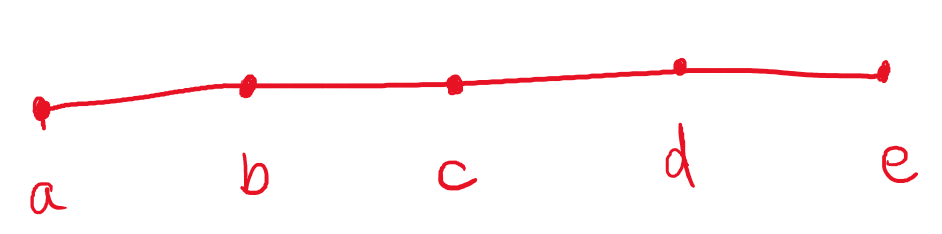
\includegraphics[scale=0.2]{./fig/ex-1.png}
\end{figure}
\[B_4(a)=\{a,b,c,d\} \subset B_3(c)=\{a,b,c,d,e\}\]
证明:若$B_7(a) \subset B_3(b)$则$B_7(a)=B_3(b)$。\\
\textbf{Proof:}
\[\forall x \in B_3(b) \ , \ d(x,a) \leq d(x,b)+d(b,a)<3+3=6<7 \ \Rightarrow \ x \in B_7(a)\]
\textbf{Q.E.D.}

\paragraph*{7.}$(X,d)$是距离空间,$A \subset X$,令$f(x)=\mathop \text{inf}\limits_{y \in A}d(x,y)$,证明$f(x)$连续。\\
\textbf{Proof:}
\[\forall x_1,x_2 \in X \ , \ y \in A \ , \ d(x_1,x_2) \leq d(x_1,y)+d(y,x_2)\]
取下极限
\[f(x_1) \leq d(x_1,x_2)+f(x_2) \ \Leftrightarrow \ f(x_1)-f(x_2) \leq d(x_1,x_2)\]
同理
\[f(x_2)-f(x_1) \leq d(x_1,x_2)\]
\[\Rightarrow \ |f(x_1)-f(x_2)| \leq d(x_1,x_2) \to 0\]
\[\forall \varepsilon>0 \ , \ d(x_1,x_2)<\delta=\varepsilon \quad \text{s.t.} \quad |f(x_1)-f(x_2)|<\varepsilon\]
\textbf{Q.E.D.}

\paragraph*{8.}证明$C^1[0,1]$是完备距离空间。\\
\textbf{Proof:}设$\{x_n(t)\}$是$C^1[0,1]$中的柯西列。
\[d(x_n(t),x_m(t))=\mathop \text{sup}\limits_{t \in [0,1]}|x_n(t)-x_m(t)|+\mathop \text{sup}\limits_{t \in [0,1]}|x_n'(t)-x_m'(t)|\]
由$C[0,1]$的完备性可知,我们只需要证明$\{x_n'(t)\}$是$C[0,1]$中的柯西列,即$x_n'(t) \rightrightarrows h(t) \in C[0,1]$。只需证
\[x_n(t) \rightrightarrows x(0)+\int_0^th(s)\dd s \qquad x(0)=\lim_{n \to \infty}x_n(0)\]
验证:
\[\left|x_n(t)-x(0)-\int_0^th(s)\dd s\right| \leq \left|x_n(0)+\int_0^tx_n'(s)\dd s-x(0)-\int_0^th(s)\dd s\right| \quad \text{微积分基本定理}\]
\[\leq \left|x_n(0)-x(0)\right|+\int_0^t|x_n'(s)-h(s)|\dd s \leq \left|x_n(0)-x(0)\right|+\mathop \text{sup}\limits_{t \in [0,1]}|x_n'(t)-h(t)| \to 0 \quad (n \to \infty)\]
且上述极限的取值与$t \in [0,1]$无关,故为一致收敛,原命题得证。\\
\textbf{Q.E.D.}

\paragraph*{8.}证明:闭球套定理成立的距离空间是完备距离空间。\\
\textbf{Proof:}原命题等价于设$(X,d)$中任一套闭球套$(r_n \to 0)$都有非空交,那么$(X,d)$完备。\\
设$\{x_n\}$是$X$中的柯西列,由它构造闭球套:
\[\forall k \in \mathbb{Z}_+ \ , \ \exists \, n_k>0 \quad \text{s.t.} \quad m,n \geq n_k \ , \ d(x_m,x_n)<\frac{1}{2^k} \ \Rightarrow \ x_n \in B_{\frac{1}{2^{k+1}}}(x_{n_k})\]
\[\Rightarrow \ \exists \, \{x_{n_k}\} \ (k=1,2,\cdots) \quad \text{s.t.} \quad \bar{B}_{\frac{1}{2^{k+1}}}(x_{n_{k+1}}) \subset \bar{B}_{\frac{1}{2^k}}(x_{n_k})\]
\[\text{由题设} \exists \,! \, x \in \bigcap_{k=1}^{\infty}\bar{B}_{\frac{1}{2^k}}(x_{n_k}) \ , \ d(x_{n_k},x) \to 0 \ (n \to \infty) \ \Rightarrow \ d(x_n,x) \to 0 \ (n \to \infty)\]
(柯西列+收敛子列$\ \Rightarrow \ $柯西列收敛)\\
\textbf{Q.E.D.}

\paragraph*{9.}设$(X,d)$完备,$\tilde{f}$为$X$上的一族连续函数,满足
\[\tilde{f}=\{F(x)|\forall x \in X \ , \exists \, M_x>0 \quad \text{s.t.} \quad |F(x)| \leq M_x\}\]

证明:$\exists \, M>0 \ , \ \exists \, U\text{(开集)} \in X \quad \text{s.t.} \quad \forall x \in U \ , \ F \in \tilde{f} \ , \ |F(x)| \leq M$\\
Proof($Baire$定理应用):设$E_n=\{x|x \in X \ , \ |F(x)| \leq n \ , \ F \in \tilde{f}\}$
\[\text{由题设} \forall x \in X \ , \ x \in E_{[M_x]+1} \ \Rightarrow \ X \subset \bigcup_{n=1}^{\infty}E_n \ \left(or \ X=\bigcup_{n=1}^{\infty}E_n \right)\]
$(X,d)$完备,由$Baire$定理,至少存在一个$M$使得$E_M$不是疏集,即存在一个开集$U \subset \bar{E}_M$
\[\forall x \in U \ , \ \exists \, \{x_n\} \subset E_M \ , \ x_n \to x \ (n \to \infty)\]
由连续性可知
\[|F(x)|=\lim_{n \to \infty}|F(x_n)| \leq M \ , \ \forall F \in \tilde{f}\]
\textbf{Q.E.D.}

\paragraph*{10.}在距离空间中证明:连续$\ \Leftrightarrow \ $开集的原像是开集。\\
Proof($\ \Rightarrow \ $):设$f:X \to Y$是连续映射,设$G \subset Y$是任一开集,要证$f^{-1}(G)$是$X$中的开集。
\[\forall x_0 \in f^{-1}(G) \ , \ f(x_0) \in G \ \Rightarrow \ \exists \, \varepsilon>0 \quad \text{s.t.} \quad B_{\varepsilon}(f(x_0)) \subset G\]
$f$是连续映射:
\[\exists \, \delta>0 \quad \text{s.t.} \quad d(y,x_0)<\delta \ , \ d_Y(f(y),f(x_0))<\varepsilon \ \Rightarrow \ f(B_{\delta}(x_0)) \subset B_{\varepsilon}(f(x_0)) \subset G\]
\[\Rightarrow \ B_{\delta}(x_0) \subset f^{-1}(G) \ \Leftrightarrow \ x_0\text{是}f^{-1}(G)\text{的内点,由}x_0\text{的任意性可得}f^{-1}(G)\text{是开集}\]
\begin{figure}[htbp]
    \center
    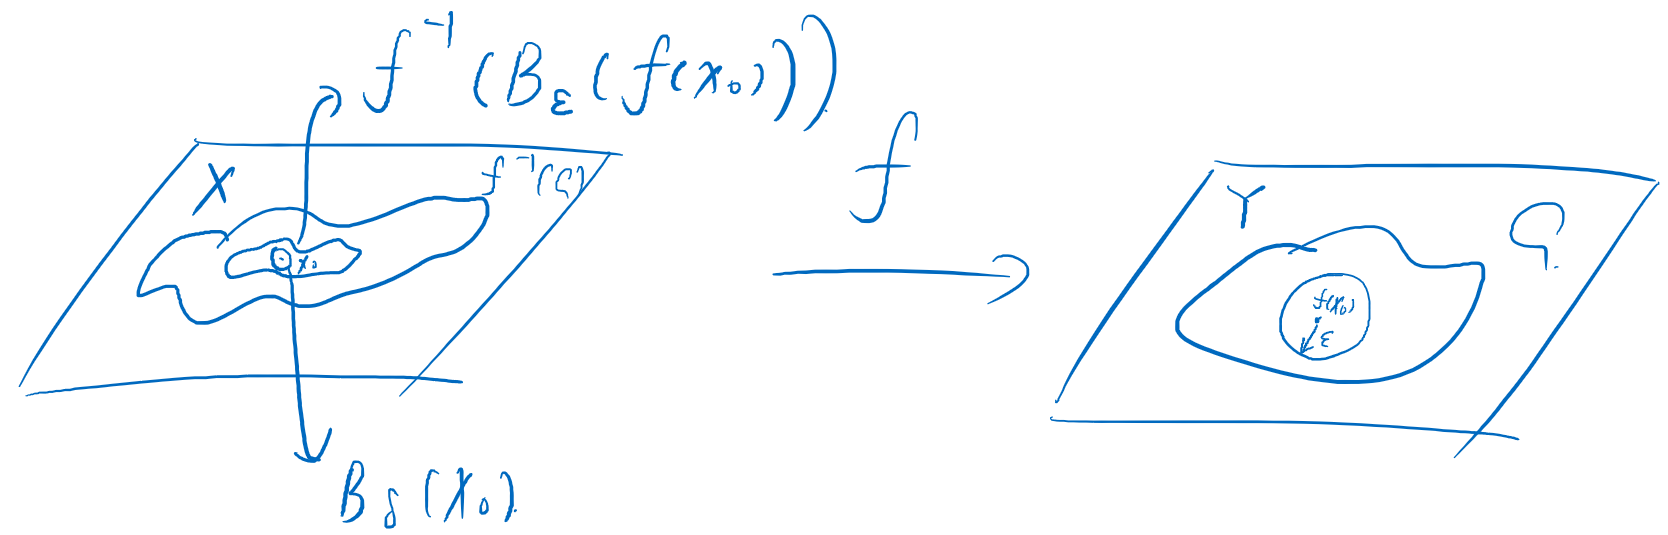
\includegraphics[scale=0.2]{./fig/ex-2.png}
\end{figure}
Proof($\ \Leftarrow \ $):设$f:X \to Y$满足开集的原像是开集,则$\forall x_0 \in X \ , \ \exists \, \varepsilon>0 \ , \ B_{\varepsilon}(f(x_0))$是$Y$中的开集。
\[\Rightarrow \ f^{-1}(B_{\varepsilon}(f(x_0)))\text{是$X$中的开集}, \ x_0 \in f^{-1}(B_{\varepsilon}(f(x_0)))\text{是内点}\]
\[\exists \, \delta>0 \ , \ f(B_{\delta}(x_0)) \subset B_{\varepsilon}(f(x_0)) \ \Rightarrow \ f\text{在}x_0\text{连续}\]
由$x_0$任意性可得$f$在$X$上连续。
\begin{figure}[htbp]
    \center
    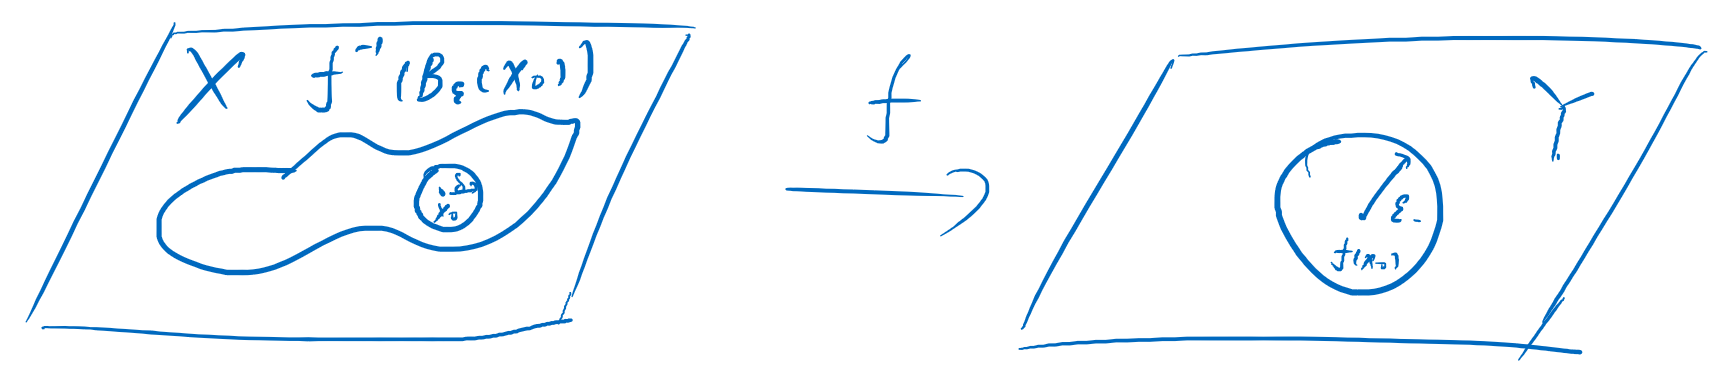
\includegraphics[scale=0.2]{./fig/ex-3.png}
\end{figure}
\textbf{Q.E.D.}

\paragraph*{11.}举例说明在压缩映射中(1)完备性不可少; \ (2)$d(Tx,Ty)<d(x,y) \ \forall x \neq y$是不充分的。
\[(1) \quad R-\{0\} \to R-\{0\} \quad x \mapsto \frac{1}{2}x \ \text{无不动点。}\]
\[(2) \quad T:[0,+\infty) \to [0,+\infty) \quad T(x)=x+\frac{1}{1+x}\]
Claim (2):
\[d(T(x),T(y))=\left|x+\frac{1}{1+x}-y-\frac{1}{1+y}\right|=\left|x-y-\frac{x-y}{(1+x)(1+y)}\right|\]
\[=\left|1-\frac{1}{(1+x)(1+y)}\right|d(x,y)<d(x,y)\]
\[T(x)=x \ \Rightarrow \ \frac{1}{1+x}=0 \ \Rightarrow \ x\text{无解,无不动点}\]
\textbf{Q.E.D.}

\paragraph*{12.}$T:X \to X \ , \ X$完备,$T$在闭球$\bar{B}_r(x_0) \ x_0 \in X$上为压缩映射,即满足
\[d(Tx,Ty) \leq \theta d(x,y) \ (\theta \in (0,1))\text{,且}d(x_0,Tx_0)<(1-\theta)r\]
证明:$T$在$\bar{B}_r(x_0)$上有唯一不动点。\\
\textbf{Proof:}只需证$T(\bar{B}_r(x_0)) \subset \bar{B}_r(x_0)$ (后续由完备闭子空间也是完备的可证)
\[\forall x \in \bar{B}_r(x_0) \ , \ d(Tx,x_0) \leq d(Tx,Tx_0)+d(Tx_0,x_0) \leq \theta d(x,x_0)+(1-\theta)r \leq \theta r+(1-\theta)r=r\]
\[\Rightarrow \ Tx \in \bar{B}_r(x_0) \ \text{由}x\text{的任意性} \ T(\bar{B}_r(x_0)) \subset \bar{B}_r(x_0)\]
把$T$限制在$\bar{B}_r(x_0)$上:$T:\bar{B}_r(x_0) \to \bar{B}_r(x_0) \ , \ T$为压缩映射,$\bar{B}_r(x_0)$是完备空间$X$上的闭子空间,所以$\bar{B}_r(x_0)$完备。由压缩映射定理即证。\\
\textbf{Q.E.D.}

\paragraph*{13.}$(t_0,s_0) \in \mathbb{R}^2 \ , \ f(t,s)$在$(t_0,s_0)$邻域$N$中连续,$s_0=f(t_0,s_0) \ , \ f_s(t,s)$在$N$中存在且在$(t_0,s_0)$连续,且$f_s(t_0,s_0)=0$。\\
证明:
\[\exists \, \delta>0 \ , \ x(t) \in C[t_0-\delta,t_0+\delta] \quad \text{s.t.} \quad x(t)=f(t,x(t)) \ , \ t \in [t_0-\delta,t_0+\delta] \ , \ x(t_0)=s_0 \ \text{有唯一解}\]
Solve:我们的思路是构造压缩映射$Tx=f(t,x(t))$来解决初值问题的证明:
\[d(Tx,Ty)=\mathop \text{sup}\limits_t|f(t,x)-f(t,y)|=\mathop \text{sup}\limits_t|f_x(t,\xi(t))||x-y| \leq \mathop \text{sup}\limits_t|f_x(t,\xi(t))|d(x,y)\]
\textbf{Proof:}
\[f_s(t,s) \in C(N) \ , \ f(t_0,s_0)=0 \ \Rightarrow \ \exists \, \delta>0 \quad \text{s.t.} \quad |t-t_0|,|s-s_0| \leq \delta \ , \ |f_s(t,s)|=\theta < 1\]
令
\[X=\{x(t) \in C[t_0-\delta,t_0+\delta] \ , \ x(t_0)=s_0 \ , \ \mathop \text{sup}\limits_{t \in [t_0-\delta,t_0+\delta]}|x(t)-s_0| \leq \frac{\delta}{2}\}\]
(极限不保严格不等号,所以上式最后一项取闭保持闭性)\\
\textbf{Claim} $X$是完备的\\
(\textbf{Proof:}$C[t_0-\delta,t_0+\delta]$是完备的,所以有
\[\forall \{x_n(t)\} \subset C[t_0-\delta,t_0+\delta] \ , \ \exists \, X_{\infty}(t) \quad \text{s.t.} \quad x_n(t) \rightrightarrows x_{\infty}(t)\]
\[\Rightarrow \ x_{\infty}(t_0)=\lim_{n \to \infty}X_n(t_0)=\lim_{n \to \infty}s_0=s_0\]
故$X$完备。\\
\textbf{Q.E.D.})\\
定义$T:X \to X \ : \ T(x(t))=f(t,x(t))$,下面验证定义良好(满足初值条件以及像在原空间中):
\[\text{1、} \ T(x(t_0))=f(t_0,x(t_0))=f(t_0,s_0)=s_0=x(t_0)\]
\[\text{2、} \ \mathop \text{sup}\limits_{t \in [t_0-\delta,t_0+\delta]}|T(x(t))-s_0|=\mathop \text{sup}\limits_{t \in [t_0-\delta,t_0+\delta]}|f(t,x(t))-s_0|=\mathop \text{sup}\limits_{t \in [t_0-\delta,t_0+\delta]}|f_s(t,\xi(t))||x-s_0| \leq \frac{\delta}{2}\]
\[\Rightarrow \ T(x(t)) \in X\]
\[d(Tx,Ty)=\mathop \text{sup}\limits_{t \in [t_0-\delta,t_0+\delta]}|f(t,x(t))-f(t,y(t))|=\mathop \text{sup}\limits_{t \in [t_0-\delta,t_0+\delta]}|f_s(t,\xi(t))||x(t)-y(t)| \leq \theta d(x,y)\]
$T$是压缩映射
\[\exists \, ! \, x(t) \in X \quad \text{s.t.} \quad x(t)=f(t,x(t))\]
\textbf{Q.E.D.}

\paragraph*{14.}证明:全有界集$A$的有限$\varepsilon$-网可取为$A$的子集。\\
这题主要用到了以下事实:
\[d(x,y)<r \ \Leftrightarrow \ x \in B_r(y) \ \Rightarrow \ B_r(y) \subset B_{2r}(x)\]
\begin{figure}[htbp]
    \center
    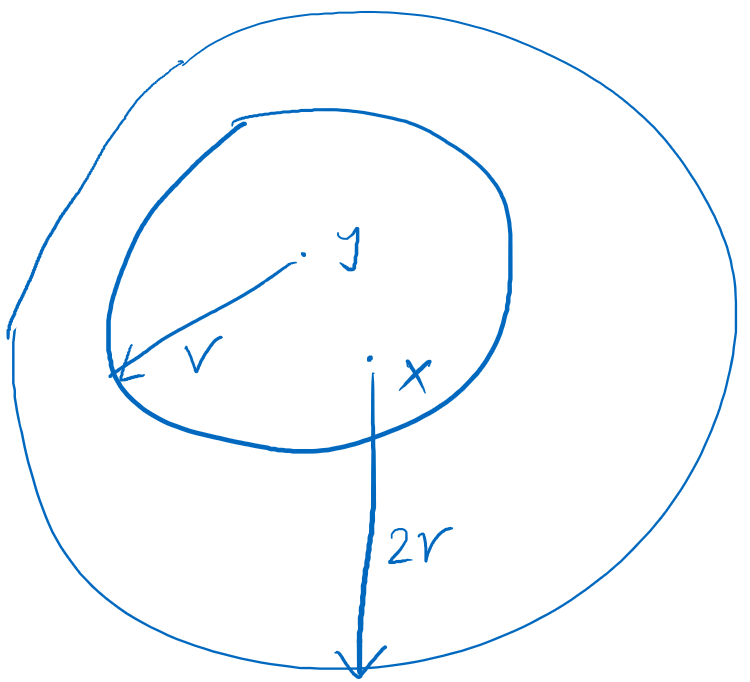
\includegraphics[scale=0.2]{./fig/ex-4.png}
\end{figure}
\textbf{Proof:}
\[\forall \varepsilon>0 \ , \ \exists \, A\text{有限}\frac{\varepsilon}{2}\text{-网} \ , \ N=\{x_1,x_2,\cdots,x_k\} \ , \ \text{若}B_{\frac{\varepsilon}{2}}(x_i) \cap A =\varnothing \ , \ \text{则可以把$x_i$从$N$中去掉}\]
\[\text{不妨设对每个} \ x_i \in N \ , \ B_{\frac{\varepsilon}{2}}(x_i) \cap A \neq \varnothing \ , \ \text{取} \ y_i \in B_{\frac{\varepsilon}{2}}(x_i) \cap A \ \Rightarrow \ B_{\frac{\varepsilon}{2}}(x_i) \subset B_{\varepsilon}(y_i)\]
\[\Rightarrow \ \tilde{N}=\{y_1,y_2,\cdots,y_k\}\text{为$A$的有限$\varepsilon$-网且} \ \tilde{N} \subset A\]
\textbf{Q.E.D.}

\paragraph*{15.}证明:$ \ C^1[0,1]$中的有界集$A$是$C[0,1]$中的相对紧集。
\begin{definition}[相对紧集]
    若集合$M$的闭包$\bar{M}$在空间中是紧集,则称$M$是相对紧集。
\end{definition}
$C[0,1]$是距离空间,故$C[0,1]$中的紧集是列紧的闭集,$\bar{A}$是闭集,故只需证明$\bar{A}$是列紧的。显然接下来我们是要利用$Arzela$定理分三步证明:

1、$A$在距离空间$C[0,1]$中有界(即一致有界); \ 2、$A$等度连续 ;\\
由1、2以及$Arzela$定理可以证明$A$是列紧的;

3、证明列紧集的闭包还是列紧的。\\
\textbf{Proof:}\\
\textbf{1.}
\[A\text{在}C^1[0,1]\text{中有界} \ \Rightarrow \ \exists \, K>0 \ , \ \forall x(t) \in A \quad \text{s.t.} \quad d_{C^1}(x(t),0) \leq K\]
\[\Rightarrow \ d_C(x(t),0) \leq d_{C^1}(x(t),0) \leq K \ \Rightarrow \ \text{$A$在距离空间$C[0,1]$中有界}\]
\textbf{2.}
\[\forall \varepsilon>0 \ , \ x(t) \in A \ , \ \exists \, t_1,t_2 \in [0,1] \quad \text{s.t.} \quad |x(t_1)-x(t_2)|=|x'(\xi)||t_1-t_2| \leq K|t_1-t_2|\]
\[\text{取} \ |t_1-t_2|<\frac{\varepsilon}{K} \ \Rightarrow \ |x(t_1)-x(t_2)|<\varepsilon\]
由1、2以及$Arzela$定理可得,$A$是列紧的;
\textbf{3.}
\[\text{任取}\{x_n(t)\}_{n=1}^{\infty} \subset \bar{A} \ \Rightarrow \ \forall x_n(t) \in \bar{A} \ , \ \exists \, y_n(t) \in A \quad \text{s.t.} \quad d_C(x_n(t),y_n(t))<\frac{1}{n}\]
因为$A$是列紧的:
\[\exists \, n_k \quad \text{s.t.} \quad y_{n_k}(t) \to y(t) \ (k \to \infty)\]
\[d_C(x_{n_k}(t),y(t)) \leq d_C(x_{n_k}(t),y_{n_k}(t))+d_C(y_{n_k}(t),y_{n_k}(t))\]
\[\leq \frac{1}{n_k}+d_C(y_{n_k}(t),y_{n_k}(t)) \to 0 \ (k \to \infty) \ \Rightarrow \ \bar{A}\text{列紧}\]
\textbf{Q.E.D.}

\paragraph*{16.}$X$是紧距离空间,$T:X \to X$是连续映射,满足$d(Tx,Ty)<d(x,y) \ \forall x \neq y$。\\
证明:$T$存在唯一不动点。

需要注意的是这里$T$不是一定压缩映射:\\
\textbf{例}
\[X=[0,1] \qquad Tx=\frac{x}{1+x}\]
\[|Tx-Ty|=\left|\frac{x}{1+x}-\frac{y}{1+y}\right|=\frac{|x-y|}{|1+x||1+y|}<|x-y| \quad (\forall x \neq y \in [0,1])\]
$T$有唯一不动点$T0=0$\\
\textbf{Proof:} 定义$f(x)=d(x,Tx)$,容易证明,$f$在$X$上连续,故由于$X$是紧集可知$f$有最小值,设$x_0$是$f$的极小值点。
\[\text{if} \ f(x_0)>0 \ \text{then} \ f(x_0) \leq d(Tx_0,T^2X_0)<d(x_0,Tx_0)=f(x_0)\]
矛盾,故$f(x_0)=0 \ \Rightarrow \ Tx_0=x_0$是不动点。\\
若$\exists \, y_0 \quad \text{s.t.} \quad Ty_0=y_0$,若$y_0 \neq x_0$,则
\[0<d(x_0,y_0)=d(Tx_0,Ty_0)<d(x_0,y_0)\]
矛盾,所有$y_0=x_0$,不动点唯一。\\
\textbf{Q.E.D.}

\paragraph*{17.}证明$Banach$空间$c_0$可分。
\[c_0=\{x=\{\xi_k\}_{k=1}^{\infty}|\lim_{k \to \infty}\xi_k=0\} \qquad ||x||=\mathop \text{sup}\limits_{k}|\xi_k|\]
\textbf{Proof:}\\
\[\text{由} \ \lim_{k \to \infty}\xi_k=0 \ \text{可知,我们可以构造下列序列组成$c_0$的子集} \ c_0'=\{x'=(\xi_i,\xi_2,\cdots,\xi_k,0,0,\cdots)\}\]
令$A=\{r=\{r_k\}_{k=1}^{\infty}|r_k \in \mathbb{Q} \ , \ \exists \, n>0 \ , \ \forall j>n \ , \ r_j=0\}$
\[\forall \varepsilon>0 \ , \ x=\{\xi_k\}_{k=1}^{\infty} \in c_0 \ , \ \lim_{k \to \infty}\xi_k=0 \ \Rightarrow \ \exists \, N>0 \ , \ \forall n \geq N \quad \text{s.t.} \quad |\xi_n|<\varepsilon\]
\[\exists \, r=(r_1,r_2,\cdots,r_N,0,0,\cdots) \in A \quad \text{s.t.} \quad ||x-r||=\mathop \text{sup}\limits_{k \in \mathbb{N}_+}|r_k-\xi_k| \leq \text{max}\left\{\mathop \text{sup}\limits_{k \in \mathbb{N}_+}|r_k-\xi_k| \ , \ \varepsilon\right\}<\varepsilon\]
因为
\[A=\bigcup_{k=1}^N\mathbb{Q} \qquad \text{card}(c_0')=\text{card}(A)=\text{card}(\mathbb{Q})\]
故$c_0$是可分的。\\
\textbf{Q.E.D.}

\paragraph*{18.}证明离散形式的$H\ddot{o}lder$不等式
\[\sum_{i=1}^n|x_iy_i| \leq \left(\sum_{i=1}^n|x_i|^p\right)^{\frac{1}{p}}\left(\sum_{i=1}^n|y_i|^q\right)^{\frac{1}{q}} \quad (p,q>0 \ , \ \frac{1}{p}+\frac{1}{q}=1 \ , \ x_i,y_i \in \mathbb{R} \ \text{or} \ \mathbb{C})\]
和$Minkowski$不等式
\[\left(\sum_{i=1}^n|x_i+y_i|^p\right)^{\frac{1}{p}} \leq \left(\sum_{i=1}^n|x_i|^p\right)^{\frac{1}{p}}+\left(\sum_{i=1}^n|y_i|^p\right)^{\frac{1}{p}} \quad (p \geq 1 \ , \ x_i,y_i \in \mathbb{R} \ \text{or} \ \mathbb{C})\]
Proof($H\ddot{o}lder$不等式):设
\[A=\left(\sum_{i=1}^n|x_i|^p\right)^{\frac{1}{p}} \qquad B=\left(\sum_{i=1}^n|y_i|^q\right)^{\frac{1}{q}}\]
由$Young$不等式:
\[\frac{|x_i| \cdot |y_i|}{A \cdot B} \leq \frac{1}{p}\frac{|x_i|^p}{A^p}+\frac{1}{q}\frac{|y_i|^q}{B^q} \ \Rightarrow \ \frac{1}{A \cdot B}\sum_{i=1}^n|x_iy_i| \leq \frac{1}{pA^p}\sum_{i=1}^n|x_i|^p+\frac{1}{qB^q}\sum_{i=1}^n|y_i|^q=1\]
\[\Rightarrow \ \sum_{i=1}^n|x_iy_i| \leq A \cdot B=\left(\sum_{i=1}^n|x_i|^p\right)^{\frac{1}{p}} \cdot \left(\sum_{i=1}^n|y_i|^q\right)^{\frac{1}{q}}\]
\textbf{Q.E.D.}\\
Proof($Minkowski$不等式):
\[\sum_{i=1}^n|x_i+y_i|^p=\sum_{i=1}^n|x_i+y_i||x_i+y_i|^{p-1} \leq \sum_{i=1}^n|x_i||x_i+y_i|^{p-1}+\sum_{i=1}^n|y_i||x_i+y_i|^{p-1}\]
\[\leq \left(\sum_{i=1}^n|x_i|^p\right)^{\frac{1}{p}}\left(\sum_{i=1}^n|x_i+y_i|^{q(p-1)}\right)^{\frac{1}{q}}+\left(\sum_{i=1}^n|y_i|^p\right)^{\frac{1}{p}}\left(\sum_{i=1}^n|x_i+y_i|^{q(p-1)}\right)^{\frac{1}{q}}\]
\[\frac{1}{p}+\frac{1}{q}=1 \ \Leftrightarrow \ p=(p-1)q\]
\[\leq \left(\sum_{i=1}^n|x_i|^p\right)^{\frac{1}{p}}\left(\sum_{i=1}^n|x_i+y_i|^{p}\right)^{1-\frac{1}{p}}+\left(\sum_{i=1}^n|y_i|^p\right)^{\frac{1}{p}}\left(\sum_{i=1}^n|x_i+y_i|^{p}\right)^{1-\frac{1}{p}}\]
\[\Rightarrow \ \left(\sum_{i=1}^n|x_i+y_i|^p\right) \cdot \left(\sum_{i=1}^n|x_i+y_i|^{p}\right)^{\frac{1}{p}-1} \leq \left(\sum_{i=1}^n|x_i|^p\right)^{\frac{1}{p}}+\left(\sum_{i=1}^n|y_i|^p\right)^{\frac{1}{p}}\]
\[\Leftrightarrow \ \left(\sum_{i=1}^n|x_i+y_i|^{p}\right)^{\frac{1}{p}} \leq \left(\sum_{i=1}^n|x_i|^p\right)^{\frac{1}{p}}+\left(\sum_{i=1}^n|y_i|^p\right)^{\frac{1}{p}}\]
\textbf{Q.E.D.}

\paragraph*{19.}设$m(E)<+\infty \ , \ f \in L^{\infty}(E)$,证明:
\[\lim_{p \to \infty}||f||_{L^p}=||f||_{L^{\infty}}\]
\textbf{Proof:}
\[||f||_{L^p(E)}=\left(\int_E|f|^p\dd t\right)^{\frac{1}{p}}=\left(\int_{E/E_0}|f|^p\dd t\right)^{\frac{1}{p}} \leq \left(m(E) \cdot ||f||^p_{L^{\infty}(E)}\right)^{\frac{1}{p}}=m(E)^{\frac{1}{p}}||f||^p_{L^{\infty}(E)}\]
\[\lim_{p \to \infty}||f||_{L^p(E)} \leq \lim_{p \to \infty}m(E)^{\frac{1}{p}}||f||^p_{L^{\infty}(E)}=||f||^p_{L^{\infty}(E)}\]
另一方面,我们令$\forall \varepsilon>0 \ , \ m(|f| \geq M-\varepsilon)=\delta>0 \ \text{where} \ M:=||f||_{L^{\infty}(E)}$
\[||f||_{L^p(E)}=\left(\int_E|f|^p\dd t\right)^{\frac{1}{p}}=\left(\int_{f \geq M-\varepsilon}|f|^p\dd t+\int_{f<M-\varepsilon}|f|^p\dd t\right)^{\frac{1}{p}}\]
\[\geq \left(\int_{|f| \geq M-\varepsilon}|M-\varepsilon|^p\dd t+\int_{|f|<M-\varepsilon}|f|^p\dd t\right)^{\frac{1}{p}} \geq |M_\varepsilon|\delta^{\frac{1}{p}}\]
由$\varepsilon$的任意性:
\[\lim_{p \to \infty}||f||_{L^p(E)} \geq \lim_{p \to \infty} |M_\varepsilon|\delta^{\frac{1}{p}}=||f||_{L^{\infty}(E)}\]
综上所述,有
\[\lim_{p \to \infty}||f||_{L^p}=||f||_{L^{\infty}}\]
\textbf{Q.E.D.}